% !TeX spellcheck = en_US
\documentclass[crop=false, class=article]{standalone}
\usepackage{pacco}
\begin{document}
\section{Introduction}
This course will deal with two main topics: \emph{Stochastic Differential Equations} (SDE) and \emph{Partial Differential Equations} (PDE). It will be mostly theoretical so fuck you. Recommended book is \textit{Brownian motion: an introduction to stochastic processes} by Renè Schilling.
\section{Introduction to stochastic differential equations: the Ito Integral}
\subsection{What is a stochastic differential equation?}
Imagine that we want to describe a \rp{} that involves time.
\begin{equation*}
	{(X_{t})}_{t\geq0}=X_{t}
\end{equation*}
Where $t\mapsto X_{t}(\omega)$. This is the evolution of our \rp{}. But what if we are interested in the \textit{variation} of the process? The we would have to consider
\begin{equation*}
	\underbrace{\dif X_{t}}_{X_{t+\dif t}-X_{t}}=c \dif t
\end{equation*}
where $c$ is a constant and $\dif t$ stands for ``an infinitesimally small amount of $t$''. Of course this notion is strictly heuristic and it is all but a rigorous definition. What the fuck does "infinitesimally small" mean anyway?\\
In this version the variation of the process is proportional to $\dt$ which is the variation of time. But what if the constant $c$ depends on the current value of $X_{t}$? Then it would become a function of $X_{t}$ and we would have
\begin{equation*}
	\dif X_{t}=c(X_{t})\dt.
\end{equation*}
Up to now there is nothing random in this. Random variables are just functions and thus are deterministic. We may want to add an aspect of randomness by adding an amount of noise dictated by the \rv{} $Y_{t}$. We may further add a coefficient $\sigma$ that tells us the amplitude of the effect of $Y_{t}$ on the variation of $X_{t}$. Of course, $\sigma$ may be dependent on the current value of $X_{t}$. So we will have
\begin{equation*}
	\dif X_{t}=c(X_{t})\dt+\sigma(X_{t})Y_{t}.
\end{equation*}
But what is $Y_{t}$? We could characterize it as a noise, that is the sum of a finite amount of quantities $Z_{n}$, each one of which affects very little $Y_{t}$ but there is a shitload of them.
\[Y_{t}\approx\sum_{k}^{n}\frac{Z_{k}}{n}\]
with $n$ approaching $\infty$. If the quantities $Z_{k}$ are independent then by the Central Limit Theorem we get
\begin{equation*}
	Y_{t}\underset{n\to\infty}{\approx}N(0,\dt).
\end{equation*} 
The mean of the normal process is generally arbitrary, unless we specifically choose a value based on some information that we have. Otherwise choose 0. The variance is proportional to the interval of time we are considering, since a bigger interval will cause the random noise to have more effect on the variation of the process.\\
We also know that in a given \brm{} $B$
\begin{equation*}
	B_{t+\dt}-B_{t}\sim N(0,\dt)
\end{equation*}
So we could write our variation as
\begin{equation*}
	\dif X_{t}=\underbracket{c(X_{t})\dt}_{\mathclap{\text{deterministic}}}+\underbracket{\sigma(X_{t})B_{t}}_{\mathclap{\text{random}}}.
\end{equation*}
We may still add more complexity by letting the constant being dependent on time:
\begin{equation*}
	\dif X_{t}=c_{t}(X_{t})\dif t+\sigma_{t}(X_{t})\dif B_{t}
\end{equation*}
but let's keep it relatively simple and try to avoid the unavoidable eerie question: \textit{this thing is totally heuristic, so this definition means absolutely nothing. What is this?}\\
Well, maybe we could take the derivative of each side...
\begin{equation*}
	\begin{array}{c}
		\dif X_{t}=c(X_{t})\dif t+\sigma(X_{t})\dif B_{t}\\
		\downarrow\\
		\frac{\dif}{\dt}X_{t}=c(X_{t})+\sigma(X_{t})\frac{\dif}{\dt}B_{t}.
\end{array}
\end{equation*}
But what the actual fuck?? We CANNOT differentiate \brm! So we need to define this quantity in another way. But first, a little refresh on integration.
	Think about the fundamental theorem of calculus:
\begin{equation*}
	X_{t}-X_{0}=\int_{0}^{t}c(X_{s})\ds+\int_{0}^{t}\sigma(X_{s})\dif B_{s}.
\end{equation*}
\begin{revise}
	When we do Riemann integrals we know that the definition is 
	\begin{equation*}
		\int_{0}^{t}f_{s}\ds=\lim_{|\Pi|\to 0}\sum_{i=1}^{f}f(x_{i})\Delta s_{i}
	\end{equation*}
	where $|\Pi|$ is the partition of the domain getting smaller and smaller up to infinitesimally fine.\\
	Recall, now the Riemann-Steltjes integral:
	\begin{equation*}
		\int_{0}^{t}f_{s}\dif f_{s}=\lim_{n\to\infty}\sum_{i=1}^{\infty}f(x_{i})\Delta f(s_{i})
	\end{equation*}
\end{revise}
	So by this notion we should be able to define the quantity
	\begin{equation*}
		\int_{0}^{t}\sigma(X_{s})\dif B_{s}
	\end{equation*}
	but we can't. Remember that $B$ is continuous but not differentiable! This is why it doesn't make sense to use it as an integrator. The Riemann-Stieltjes integral is computed by weighing the function by the variation of the integrator, but the \brm{} has unbounded variation (this is why it doesn't have any derivative) so it doesn't make sense to use it to weigh another function. \\
	This is why we need a new defintion of integral: the \emph{It\^o integral}.
Consider the \textit{parabolic differential equation}:
\begin{equation*}
	\frac{\partial}{\partial t}q(x,t)=Lq(x,t)\qquad\text{with }q(x,0)=u(x),\;x\in\R.
\end{equation*}
Typically 
\begin{equation*}
	L=a(x)\frac{\partial}{\partial x}+b(x)\frac{\partial^{2}}{\partial x^{2}}.
\end{equation*}
Parabolic differential equations are typically used to model the behavior of heat waves or particle dispersion. $a(x)$ is normally advection (or transport) and $b(x)$ is normally the diffusion rate. What is important is that in order for it to be a parabolic differential equation the term $L$ has to contain first and second partial differentials.\\
The problem is that there is no analitical solution $q(x,t)$ such that
\begin{equation*}
	\frac{\partial}{\partial t}q(x,t)=\frac{\partial^{2}}{\partial x^{2}}q(x,t)
\end{equation*}
as it is often the case with heat equations, but we can write it using expectation:
\begin{equation*}
	q(x,t)=\ev_{X}u(X_{t})
\end{equation*}
which is basically the multiplication of the expected value of the process by its initial condition. It is like... the average of the random process! The connection here should be
\begin{equation*}
	\arraycolsep=1.4pt
	\begin{array}{cccccc}
		\dif X_{t}&=&b(X_{t})&\dt+&\sigma(X_{t})&\dif B_{t}\\
		&&\uparrow&&\uparrow&\\
		L&=&a(X)&\frac{\partial}{\partial x}+&b(X)&\frac{\partial^{2}}{\partial X^{2}}
	\end{array}
\end{equation*}
But how is $q(x,t)=\ev_{X}u(X_{T})$ useful to us? Well, thinking about Monte-Carlo methods we can say that
\begin{equation*}
	q(x,t)\approx\frac{1}{N}\sum_{t=1}^{N}u(X^{\star}_{t})
\end{equation*}
where we simulate the process $N$ times in order to get $X^{\star}$ and do the average. \\
In general, applying numerical schemes to 
\begin{equation*}
	b(X_{t})\dt+\sigma(X_{t})\dif B_{t}
\end{equation*}
is much easier than applying them to L.
\subsection{Revising \brm}
Take $(E,\E)$ and $(F,\F)$ being two measurable spaces. Then
\begin{equation*}
	E\times F+\{(x,y):x\in E,y\in R\}.
\end{equation*}
Now take $A\subset E,B\subset F$ and $x\in A,y\in B$. Then
\begin{equation*}
	\E\otimes\F=\sigma(\text{measurable rectangles})
\end{equation*}
so if we take $A\in\E$ and $B\in\F$, $A\times B$ is a measurable rectangle. Now for our purposes we have to generalize it to infinite dimensions.\\
Consider an arbitrary set $T$ such that $T=[0,\infty)$ and that for each $t$ $(E_{t},\E_{t})$ is a measurable space. Take $X_{T}\in E_{t}\;\every t\in T$. Then then sequence ${(X_{t})}_{t\in i}$ is a function on $T$: $T\ni t\mapsto X_{t}\in E_{t}$, with $E_{t}$ being always the same so $E_{t}=E\;\every t$.\\
So take $F:=\{\text{the set of all such function}\}$ (that is, the product space). A rectangle in $F$ is the subset
\[\bigtimes_{t\in T}A_{t}=\{X\in F:X_{t}\in A_{t}\every t\in T\}\]
where $A_{t}$ differs from $E$ only in a finite number of $t$. It's like a rectangle is a set of functions with only a finite number of prescribed positions.
\begin{figure}[H]
	\centering
	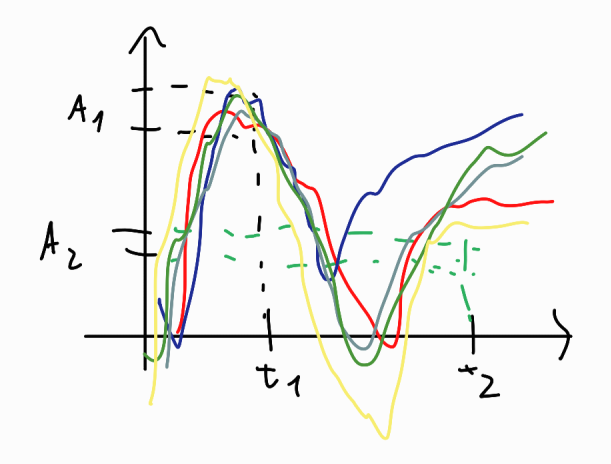
\includegraphics[width=0.7\linewidth]{images/screenshot001}
	\caption{The rectangle in the product space is the finite number of functions that pass by the two rectangle in the drawing.}
	\label{fig:screenshot001}
\end{figure}
The rectangle is measurable if $A_{t}\in\E_{t}$ for $\every t\in T$.
\begin{equation*}
	\bigotimes_{t\in T}\E_{t}=\sigma(\text{measurable rectangles}).
\end{equation*}
Take $E=\R,T=(0,\infty]$ so that our space becomes $(\R^{(0,\infty]},\B((0,\infty]))$ so that the information in our product \sa{} evokes a finite number of positions. This is really important for considering trajectories.
\begin{proposition}
	Let $(\Omega,\mathcal{A})$ be measurable. For each $t\in T$ let $f_{t}:\Omega\mapsto E_{t}$. For each $\omega\in\Omega$ define $f(\omega)$ as the point ${\big(f_{t}(\omega)\big)}_{t\in T}$ in $F$. Then $f:\Omega\mapsto F$ is $\mathcal{A}$-measurable if and only if $f_{t}$ is $\mathcal{A}$-measurable for $\every t\in T$.
\end{proposition}
We also need the notion of \emph{\brm}:
\begin{revise}
	A $d$-dimensional process ${(B_{t})}_{t\geq0}=B$ is a \brm{} on $(\Omega,\mathcal{A},\pr)$ if:
	\begin{itemize}
		\item $B_{0}=0$;
		\item it has independent increments:
		\begin{equation*}
			B_{t_{i}}=B_{t_{i-1}}\text{ is independent }i=1,\ldots,n\;\every n\in\N;
		\end{equation*}
		\item it has stationary incrememnts: taking $0\leq s\leq 1$ brings us to 
		\begin{equation*}
			B_{t}-B_{s}\sim B_{t-1};
		\end{equation*}
		\item gaussianity:
		\begin{equation*}
			B_{t}-B_{s}\sim N(0,(t-s)\indi);
		\end{equation*}
		$t\mapsto B_{\omega}$ are continuous for all $\omega\in\Omega$.
	\end{itemize}
\end{revise}
	How are we sure that this object exists? The answer would be Kolmogorov's theorem but we cannot use it because we can only use with product \sa s which is not the case.
	ctually, to construct and prove the existence of the BM there are two approaches:
	\begin{itemize}
		\item the \textbf{Lévy construction}, which only works for the Brownian Motion
		\item the \textbf{canonical construction}, which is used for many processes and consists in fixing a probability space $(C_0(I)), \ldots, \ldots)$ with $C_0(I)$ space of continuous functions, then identifying a $\sigma$-algebra and a probability measure to obtain a BM. To do so, we use $X(\omega) = \omega$ as a process.
	\end{itemize}
	We want to find a probability space $(\Omega, \mathcal{F}, \mP)$ and a r.v. on it satisfying the definition. The Kolmogorov Theorem allows to do it. Recall first that we are going to work with 
	\begin{equation*}
		\mathbb{R}^I = \{\omega: I \to \mathbb{R}\} = \bigtimes _{t \in I} \mathbb{R}, \quad \B^I(\mathbb{R}) = \bigtimes_{t \in I} \quad \text{ product $\sigma$-algebra }
		\B(\mathbb{R})
	\end{equation*}
	considering therefore the space $(\mathbb{R}^I, \B^I(\mathbb{R}))$.
	\begin{theorem}[Kolmogorov Theorem]
		For each $t_1, \dots, t_n \geq 0$ and for every $n \in \mathbb{N}, $ with $t_j \neq t_k$, $j \neq k$, let $p_{t_1, \dots, t_n}(\cdot, \dots, \cdot)$ be a probability measure on $(\mR^n, \B(\mR^n))$ (for fixed times $t_i$). \\
		Assume that this family satisfies the so-called consistency conditions:
		\begin{enumerate}
			\item $p_{t_1, \dots, t_n}(A_1 \times  \dots \times  A_n) = p_{t_{\sigma(1)}, \dots, t_{\sigma(n)}}(A_{\sigma(1)} \times  \dots \times  A_{\sigma(n)})$ where $\sigma:\{1, \dots, n\} \to \{1, \dots, n\} $ is a permutation of $\{1, \ldots, n\}$;
			\item $p_{t_1, \dots, t_{n-1}}(A_1\times  \dots \times  A_{n-1}) =p_{t_1, \dots, t_{n-1}, t_n}(A_1\times  \dots \times  A_{n-1}\times \mR) $
		\end{enumerate}
		Then there exists a (unique) probability measure $\mu$ on the product space $(\mR^{[0,\infty)}, \B^{[0,\infty)}(\mR))$ such that the canonical process $X=(X_t)_{t \geq 0}$ with $X_t(\omega)= \omega(t)$ has finite dimensional distribution 
		\begin{equation*}
			\mP(X_{t_1}\in A_1, \dots, X_{t_n} \in A_n)= p_{t_1, \dots, t_n}(A_1 \times \dots \times  A_n)
		\end{equation*}
		for any $t_1, \dots, t_n$, $n \in \mathbb{N}$.
	\end{theorem}
	\begin{corollary}
		There exists a unique measure $\mu$ on $(\mR^I,\B^I(\mR) )$ such that the canonical process $X=(X_t)_{t \geq 0}$ satisfies $X_0=0$ almost surely, has  stationary and independent increments. 
	\end{corollary}
	\begin{fancyproof}[Sketch of the proof]
		This is just a sketch of the proof.
		Let $p_{t_1, \dots, t_n}$ be Gaussian $(\underline{0}, C)$, $C_{ij}= min(t_i, t_j)$. The Gaussian distribution satisfies the consistency conditions. 
	\end{fancyproof}
	Now, the next thing we need is the continuity of trajectories. Define
	\begin{equation*}
		C_0=\{\omega \in \mathbb{R}^I \text{s.t. } \omega \text{ is continuous and } \omega(0) = 0\}
	\end{equation*}
	We would like to have $\mu(C_0) = 1$, but we are not sure about its validity. The problem is that the product $\sigma$-algebra is too small and the Kolmogorov theorem holds on the product $\sigma$-algebra.
	\begin{lemma}
		For every $I \in \B^I(\mathbb{R})$ there exists on at most countable set $S \subset [0,+\infty)$ s.t. $v \in I, \omega \in \mathbb{R}^I, v|_S = \omega |_S$, then $\omega \in I$. 
	\end{lemma}
	Therefore, $C_0 \notin \B^{[0,+\infty)}$. So, not all the elements contain continuous functions and hence we cannot compute the probability $\mu(C_0)$. The solution to this problem is provided by the following theorem.
	\begin{theorem}[Kolmogorov-Centsov]
		Let \((X_t)_{t \geq 0}\) be a \(d\)-dimensional process in \((\Omega, \mathcal{F}, \mathbb{P})\). If there are constants \(c > 0\), \(\alpha > 0\), and \(\beta > 0\) such that:
		\begin{equation*}
			\mathbb{E} \left( |X_t - X_s|^\alpha \right) \leq c |t - s|^{1 + \beta}, \quad \text{for all } s, t \geq 0
		\end{equation*}
		then \(X_t\) has a version with exclusively only continuous trajectories.
	\end{theorem}
	Recall that a version of a process is a process itself $(Y_t)_{t \geq 0}$ such that 
	\begin{equation*}
		\mathbb{P}(X_t = Y_t) = 1 \quad \text{ for all } t \geq 0
	\end{equation*}
	\begin{equation*}
		\begin{split}
			& (\mathbb{R}^{[0, +\infty)}, \B^{[0,+\infty)}(\mathbb{R}), \mu) \quad X \rightarrow Y \\
			& Y: \mathbb{R}^{[0,+\infty)} \hookrightarrow C_0 \\
			& (C_0, \B(C_0), \mathbb{P})
		\end{split}
	\end{equation*}
	If we put together these two results we get the continuity of trajectories! \\
	Take $(\mathbb{R}^I, \B^I(\mathbb{R}), \mu)$ and use $Y=(Y_t)_{t \in I}$ which is the Kolmogorov-Centsov version of the canonical process on $(\mathbb{R}^I, \B^I(\mathbb{R}))$. Then, take $(C_0(I), \B(C_0(I)), P)$ where $P$ is the Wiener measure and $B = (B_t)_{t \geq 0}$ is the canonical process on $(C_0(I), \B(C_0(I)), P)$. 
	\subsection{Properties of the Brownian Motion}.
Consider a function $f:[0,+\infty) \rightarrow \mathbb{R}$ and suppose we want to know the distance run by $f$ on $[0,t]$. 
\begin{equation*}
	|f(t_1) - f(t_0)|+|f(t_2) - f(t_1)|+ \ldots
\end{equation*}
approximated this distance. The approximation is clearly rough but we try to improve it by letting the length of the subintervals go to $0$. 
\begin{definition}
	Let $f:[0,+\infty) \to \mathbb{R}$ be a function on $\Pi := \{0 = t_0 < t_1 < \ldots < t_n = t\}$, a partition of $[0,t]$ with mesh $|\Pi| := \max_j |t_j - t_{j-1}|$. For $p > 0$ we call 
	\begin{align*}
		S_p^\Pi(f,t) &= \sum_{t_j \in \Pi} |f(t_j) - f(t_{j-1})|^p\\
		&= \sum_{j=1}^n |f(t_j) - f(t_{j-1})|^p
	\end{align*}
	is the p-variation sum of $f$ along $\Pi$. 
\end{definition}
We call $VAR_p(f,t) := \sup\{S_p^\Pi(f,t): \Pi \text{ permutation of } [0,t]\}$ the strong p-variation.\\
$VAR_1(f,t) < \infty$, then $f$ is of bounded variation.  
\begin{definition}[$p$-variation]
	Let \( f \colon [0, \infty) \to \mathbb{R} \) and let \( (\Pi_n)_{n \in \mathbb{N}} \) be a sequence of partitions of \([0, t]\) with \( |\Pi_n| \to 0 \) as \( n \to \infty \). 
	
	Then, the \(p\)-variation of \(f\) over \([0,t]\) is defined as:
	
	\[
	\text{Var}_p(f, t) := \lim_{n \to \infty} S_p^{\Pi_n}(f, t)
	\]
	
	where \( S_{\Pi_n}(f, t) \) denotes the sum associated with the partition \(\Pi_n\).
\end{definition}
We want $f$ to be the Brownian Motion, depending on the trajectories:
\begin{equation*}
	f_t \equiv B_t(\omega)   
\end{equation*}
The main result is the following.
\begin{theorem}
	Let $(B_t)_{t \geq 0}$ be a Brownian Motion. Let $(\Pi_n)_{n \in \mathbb{N}}$ be a sequence of partitions of $[0,t]$ s.t. $|\Pi_n| \rightarrow 0$. Then
	\begin{equation*}
		VAR_2(B,t) := L^2-\lim_{n \rightarrow +\infty} S_2^{\Pi_n}(B,t) = t
	\end{equation*}
\end{theorem}
This means that the quadratic variation of the Brownian Motion equals $t$ in the $L^2$ sense. 
\begin{proof}
	The thesis is 
	\begin{equation*}
		\lim_{|\Pi| \rightarrow 0} \mathbb{E}|S_2^\Pi(B,t) - t|^2 = 0
	\end{equation*}
	with $\Pi = \{0 = t_0 < t_1 < \ldots < t_n = t\}$.
	\begin{equation*}
		\mathbb{E}(S_2^\Pi(B,t)) = \sum_{j=1}^n \mathbb{E}(B{t_j} - B_{t_j-t_{j-1}})^2 = \sum_{j=1}^n(t_j-t_{j-1}) = t
	\end{equation*}
	
	\begin{align*}
		\mathbb{E}(S_2^\Pi(B,t)-t)^2 &= \mathbb{V}ar(S_2^\Pi(B,t)) \\
		&= \sum_{j=1}^{n} \mathbb{E} [(B_{t_j} - B_{t_{j-1}})^2 - (t_j - t_{j-1})]^2 \\
		&= \sum_{j=1}^{n} \mathbb{E} [B^2_{t_j - t_{j-1}} - (t_j - t_{j-1})]^2 \\
		&= \sum_{j=1}^{n} (t_j - t_{j-1})^2 \mathbb{E} [B_1^2 - 1]^2 \\
		&\leq c \sum_{j=1}^{n} (t_j - t_{j-1}) (t_j - t_{j-1}) \\
		& \leq c \underbrace{|\Pi| }_{\text{ bound with maximum }} \sum_{j=1}^{n} |t_j - t_{j-1}| = c |\Pi| t \rightarrow 0 \quad |\Pi| \rightarrow 0
	\end{align*}
\end{proof}
\begin{proposition}
	\begin{equation*}
		S_2^{\Pi_n}(B,t) \xrightarrow{L^2} t
	\end{equation*}
	There exists $(\Pi_{n_k})_{k \in \mathbb{N}}$ s.t. $S_2^{\Pi_{n_k}} (B,t) \xrightarrow{ \text{ a.s. }} t$.
\end{proposition}
For example, 
\begin{equation*}
	\sum_n |\Pi_n| < +\infty
\end{equation*}
then $S_2^{\Pi_n}(B,t) \xrightarrow{ \text{a.s.}} t$.
\begin{proposition}
	\begin{equation*}
		VAR_p(B,t) = +\infty \text{  a.s. } \forall t \geq 0, p \leq 2
	\end{equation*}
\end{proposition}
For $p=2$ it is possible to find $\Pi_n(\omega)$ s.t. $\lim_{n\rightarrow +\infty} S_2^{\Pi_n(\omega)} (B,t) = +\infty$.\\
The idea is that if we consider the distance $|b-a| > 0$ of only one trajectory we get a very bad approximation, while if instead we take all the trajectories in average we obtain a pretty good approximation in  $L^2$. 
\begin{equation*}
	\int_0^t f dg := \lim_{|\Pi| \rightarrow 0} \sum_{t_j \in \Pi} f(\xi_j)(g(t_j) - g(t_{j-1})
\end{equation*}
with $\xi_j \in [t_{j-1}, t_j)$. If we transform it into an $L^2$ integral adding the dependence on $\omega$, then the integral now converges. This is not the true definition of Ito integral though, of which we will give an easier approach later. 
\begin{definition}
	A function $f:[0,+\infty) \rightarrow \mathbb{R}$ is said to be locally Holder continuous of order $\alpha \in (0,1]$ if, for every $T>0$, there is a constant $c(T)$ s.t.
	\begin{equation*}
		|f(t)-f(s)| \leq c|t-s|^\alpha \quad s,t \in [0,T]
	\end{equation*}
\end{definition}
The function is globally Holder continuous if $c(T) = c$ does not depend on T. 
\begin{theorem}
	Almost all Brownian paths are nowhere locally Holder-continuous for $\alpha>\frac{1}{2}$.
\end{theorem}
\begin{fancyproof}
	Fix $\alpha > \frac{1}{2}$. Take $I=[a,b]$. Define 
	\begin{equation*}
		\mathcal{N}_{a,b} := \{\omega \in \Omega: \exists c(\omega) \text{  s.t.  } |B(t,\omega) - B(s,\omega)| \leq c(\omega) |t-s|^\alpha \forall s,t \in [a,b]\}
	\end{equation*}
	We want to prove
	\begin{equation*}
		\mathbb{P}(\cup_{a,b} \mathcal{N}_{a,b}) = 0
	\end{equation*}
	Since $a,b \in [0,+\infty)$ they can be rationals, making the unione countable. Therefore, since
	\begin{equation*}
		\mathbb{P}(\cup_{a,b} \mathcal{N}_{a,b}) \leq \sum_{a,b \in \mathbb{Q}}\mathbb{P}(\mathcal{N}_{a,b})
	\end{equation*}
	we need to prove $\mathbb{P}(\mathcal{N}_{a,b})=0$. Fix $\omega \in \mathcal{N}_{a,b}$ and suppose by contradiction the function is Holder continuous of order $\alpha$. 
	\begin{align*}
		S_2^{\Pi_n}(B(\cdot,\omega), [a,b]) &= \sum_{j=1}^n (B_{t_j}(\omega) - B_{t_{j-1}}(\omega))^2\\
		&\stackrel{\omega \in \mathcal{N}_{a,b}}\leq c^2(\omega) \sum_{j=1}^n |t_j - t_{j-1}|^{2\alpha+1-1} \\
		&\leq c^2(\omega) |\Pi|^{2\alpha -1} \sum|t_j-t_{j-1}| \rightarrow 0 \quad |\Pi| \rightarrow 0 
	\end{align*}
	We know that there exists a sequence $(\Pi_n)_{n \in \mathbb{N}} $ of partitions of $[a,b]$ s.t. $|\Pi_n| \rightarrow 0$ and $S_2^{\Pi_n}(B, [a,b]) \xrightarrow{ \text{ a.s. }} b-a$. This leads to a contradiction. 
\end{fancyproof}
We are now trying to use this regularity in $L^{2}$ to our advantage.
\begin{theorem}
	Let ${(X_{t})}_{t\geq0}$ be a \rp{} on $\R$ with continuous paths. Let $T>0$. If there exists finite constants $c>0$ and $\beta,\gamma>0$ such that
	\begin{equation*}
		\ev|X_{t}-X_{s}|^{\gamma}\leq c|t-s|^{1+\beta}\qquad s,t\in[0,T].
	\end{equation*}
	Then the paths $[0,T]\ni t\mapsto X_{t}(\omega)$ are almost surely Hölder continuous of order $\alpha\in(0,\frac{\beta}{\gamma})$ and
	\begin{equation*}
		\ev\left[\sup_{\substack{0<|s-t|<1 \\ s,t\in[0,T]}}\frac{|X_{t}-X_{n}|}{|t-s|^{\alpha}} \right]^{\gamma}<+\infty\qquad\alpha\in\left(0,\frac{\beta}{\gamma}\right).
	\end{equation*}
\end{theorem} 
This is basically a weaker version of the Kolmogorov-Chensov theorem: here we are only assuming continuity.
\begin{corollary}
	The trajectories $t\mapsto B_{t}(\omega)$ of a \brm{} are almost surely locally Hölder for $\alpha<\frac{1}{2}$.
\end{corollary}
\begin{fancyproof}
	\begin{equation*}
		\ev|B_{t}-B_{s}|^{n}\underset{\text{stationarity}}{=}\ev|B_{t-s}|^{n}\underset{\text{scaling}}{=}|t-s|^{\frac{n}{2}}\underbracket[0.6pt]{\ev|B_{t}|}_{\text{constant}}
	\end{equation*}
	and therefore
	\begin{equation*}
		\ev|B_{t}-B_{s}|^{\gamma}=c|t-s|^{1+\beta}.
	\end{equation*}
	Set $\gamma=n$ and $\beta=\frac{n}{2}-1$ so that
	\begin{equation*}
		\alpha<\frac{\beta}{\gamma}=\frac{1}{2}-\frac{1}{n}
	\end{equation*}
	and for $n$ big enough we can get the desired value.
\end{fancyproof}
\begin{proposition}
	For each fixed $T>0$ the Brownian paths $t\mapsto B_{t}(\omega)$ are not differentiable at $t=T$ \as{}
\end{proposition}
But this is not strong enough. What about, instead, this?
\begin{proposition}
	The sample paths $t\mapsto B_{t}(\omega)$ are,\as, nowhere differentiable (proof in Toaldo's notes).
\end{proposition}
Well, we know that  \brm{} has almost surely unbounded total variation so that if we take any interval the variation of the paths diverges. Let's be more specific.
\begin{proposition}
	With probability 1 there is no interval $[a,b]\subset(0,\infty)$ where $t\mapsto B_{t}$ is monotone.
\end{proposition}
This means that we canno pick an interval where the trajectory is always (weakly) decreasing or increasing. This is related to the \textit{fractal property} of \brm.\\
\subsection{Defining the Ito integral}
But why did we spent al of this time with Brownian motion? Remember that we want to arrive at the point where we study
\begin{equation*}
	\begin{array}{ccc}
		\dif X_{t}&=b_{t}(X_{t})\dt&+\sigma_{t}(X_{t})\dif B_{t}\\
		&\downarrow&\\
		X_{t}-X_{0}&=\int_{0}^{t}b_{s}(X_{s})\ds&+\int_{0}^{t}\sigma_{s}(X_{s})\dif B_{s}\\
		&&\downarrow\text{fix a trajectory}\\
		&&\int_{0}^{t}\sigma_{s}(X_{s}(\omega))\dif B_{s}(\omega).
	\end{array}
\end{equation*}
Yeah but... could this work?
\begin{revise}
	We have an interval $I:(a,b)$ and a function $f:[a,b]\mapsto\R$. We add a partition
	\begin{equation*}
		\Pi_{n}:\{a=x_{0}<x_{1}<\ldots<x_{n}=b\}
	\end{equation*}
	and take
	\begin{equation*}
		\sum_{j=0}^{n-1}f(\xi_j)(x_{j+1}-x_{j})\qquad\xi_{j}\in[x_{j},x_{j+1}].
	\end{equation*}
	Take the mesh $|\Pi_{n}|$ to the limit $n\to0$. If the limit exists and it is a constant $c$ then the \emph{Riemann integral} is defined as
	\begin{equation*}
		\int_{a}^{b}f(t)\dt:=c.
	\end{equation*}
	Remember the conditions of existence for Riemann integrals: $f$ must be continuous in $[a,b]$. \\
	If we integrate a function against another one (let's say $g(x)$) then we obtain the \emph{Riemann-Stieltjes integral}. We have
	\begin{equation*}
		\int_{a}^{b}f(t)\dif g(t)=\lim_{|\Pi|\to 0}\sum_{j=0}^{n-1}f(\xi_j)(g(x_{j+1})-g(x_{j}))\qquad\xi_j\in[x_{j},x_{j+1}].
	\end{equation*}
	For the Riemann-Stieltjes integral to exists there must be no discontinuities in both $g$ and $f$ (that is $f\circ g$) at the same point $x$. The sufficient condition is that $f$ is continuous and $g$ is of bounded variation.
\end{revise}
So how is this useful to our integral?
\begin{equation*}
	\int_{0}^{t}\underbrace{\sigma_{s}(X_{s})}_{\mathclap{\text{this may be continuous}}}\dif \overbrace{B_{s}}^{\mathclap{\text{this is NOT of bounded variation}}}
\end{equation*}
So we have necessary conditions but not sufficient conditions! It is however reasonable to require that $\int_{0}^{t}f(s)\dbs$ exists for any $\mathcal{C}[0,T]$. There is a problem, though.
\begin{proposition}
	Let $\alpha:[a,b]\mapsto\R$ be a real valued function and denote
	\begin{equation*}
		I(f):=\int_{a}^{b}f(t)\dif\alpha(t).
	\end{equation*}
	If $I(f)$ exists as a Riemann-Stieltjes integral for all $f\in\mathcal{C}[a,b]$ then $\alpha$ is of bounded variation.
\end{proposition}
Remember that this means that 
\begin{equation*}
	\norm{\alpha}_{\mathrm{TV}}:=\sup_{\Pi}\sum_{t_i\in\Pi}|\alpha(t_{i}()-\alpha(t_{i}-1)|<\infty.
\end{equation*}
The problem is that \brm{} is never of bounded variation so we can't use Riemann-Stieltjes. The integral \textit{could} exist but it does not generally exists. Consider, for instance, $\int_{0}^{t}B_{s}\dbs$. Of course this shit doesn't exist.
To prove this claim we need to recall a theorem from real analysis.
\begin{revise}
	This is the \emph{Banach-Steinhaus theorem}. Let $(X,\norm{\cdot}_{X})$ and $(Y,\gnorm{Y})$ be Banach spaces. Let $I$ be any index set. For each $i\in I$ let $S_{i}:X\mapsto Y$ be a continuous linear map. If
	\begin{equation*}
		\sup_{i\in I}\norm{S_{i}(X)}_{Y}<\infty\qquad x\in X
	\end{equation*}
	then
	\begin{equation*}
		\sup_{i\in I}\underbrace{\sup_{\norm{X}_{X}\leq1}\norm{S_{i}(X)}_{Y}}_{\text{operator norm}}<\infty.
	\end{equation*}
\end{revise}
\begin{fancyproof}
	In our proof $X=\mathcal{C}([a,b])$ (which is a Banach space), $\gnorm{X}=\gnorm{\infty}$, $Y=\R$, $\gnorm{Y}=|\cdot|$. $I$ is family of all finite partitions of $[a,b]$. Take a partition $\Pi\in I$ on which we define the operator depending on $\Pi$
	\begin{equation*}
		S_{\Pi}(f):=\sum_{i=1}^{n}f(t_{i})(\alpha(t_{i})-\alpha(t_{i-1}))\qquad f\in\mathcal{C}([a,b])
	\end{equation*}
	which clearly is a linear map. We want to check that we can apply Banach-Steinhaus by controlling that we can compute the norm
	\begin{align*}
		|S_{\Pi}(f)|&\leq\norm{f}_{\infty}\underbrace{\sum_{i=1}^{n}|\alpha(t_{i})-\alpha(t_{i-1})|}_{\text{constant}}\\
		&=c_{\Pi,\alpha}\norm{f}_{\infty}<\infty.
	\end{align*}
	Bounded operators are continuous so $S_{\Pi}$ is a continuous linear map for every index. By assumption we know that
	\begin{equation*}
		S_{\pi}(f)\xrightarrow[\Pi\to0]{}\int_{a}^{b}f(t)\dif\alpha(t)\qquad\every f\in\mathcal{C}[a,b]
	\end{equation*}
	so that
	\begin{equation*}
		\sup_{\Pi}|S_{\Pi}(f)|<\infty.
	\end{equation*}
	Imagine that this quantity goes to infinite. Then it must be infinite necessarily for a mesh going to 0, since for any other mesh it is only a finite sum of number and as such cannot be infinite. So by Banach-Steinhaus theorem
	\begin{equation*}
		\sup_{\Pi}\sup_{\norm{f}_{\infty}\leq1}|S_{\Pi}(f)|<\infty.
	\end{equation*}
	To prove the claim we must show that
	\begin{equation*}
		\norm{\alpha}_{\mathrm{TV}}<\infty
	\end{equation*}
	but if we manage to express the total variation as one of those statement we are done.
	\begin{align*}
		\norm{\alpha}_{\mathrm{TV}}&=\sup_{\Pi}\sum_{i=1}^{n}|\alpha(t_{i})-\alpha(t_{i-1})|\\
		&\sup_{\Pi}S_{\Pi}(f_{t_i}).
	\end{align*}
	Imagine a function between -1 and 1:
	\begin{figure}[H]
		\centering
		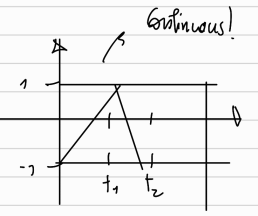
\includegraphics[width=0.4\linewidth]{resources/screenshot001}
		\label{fig:screenshot001}
	\end{figure}
	If $|\alpha(t_{i})-\alpha(t_{i+1})|$ is positive then also $f$ must be positive as it is its absolute value. $f$ is then piece-wise linear with 
	\begin{align*}
		f_{\Pi}(t_{i}) & =\mathrm{sign}(\alpha(t_{i})-\alpha(t_{i+1}))\\
		 & \leq\sup_{\Pi}\sup_{\norm{f}_{\infty}\leq1}|S_{\Pi}(f)|<\infty.
	\end{align*}
	Since \brm s are not of bounded variation a.s., $\int_{0}^{T}f(t)\dbs$ cannot be defined as a Riemann-Stieltjes integral if the class of admissible integrands contains all continuous functions $f$ on $[0,T]$.
\end{fancyproof}
We need to change the mode of convergence. $\lim_{|\Pi|\to 0}\sum_{t_i\in\Pi}f(t_{i})(B_{t_{i+1}}-B_{t_{i}})$ is very likely to be $\infty$ for $f\in\mathcal{C}([a,b])$. But consider the $L^{2}$ limit for $|\Pi|\to0$. Could this be different? Revise how the Lebesgue integral is defined.
\begin{revise}
	Take $f$ simple. Then
	\begin{equation*}
		\int_{E}f(t)\dt=\sum_{i=1}^{n}a_{i}|t_{i}-t_{i-1}| \qquad t_{i}\in\Pi
	\end{equation*}
	with
	\begin{equation*}
		f=\sum_{i=1}^{n}a_{i}\indi_{(t_{i-1},t_{i})}(t)\geq0.
	\end{equation*}
	Given $f\geq0$ measurable then $\exists f_{n}\nearrow f$ and we find
	\begin{equation*}
		\int_{a}^{b}f\dt=\lim_{n}\int_{a}^{b}f_{n}\dt.
	\end{equation*}
	if $f$ is not positive I take the canonical decomposition
	\begin{equation*}
		f=f^{+}-f^{-}
	\end{equation*}
	and take
	\begin{equation*}
			\int_{a}^{b}f\dt=	\int_{a}^{b}f^{+}\dt-	\int_{a}^{b}f^{-}\dt.
	\end{equation*}
	If both are $\infty$ then the Lebesgue integral is undefined.
\end{revise}
The Ito integral is similar, but we can't use pointwise operations due to the fact that we are dealing with a \brm{}. We need to adapt this construction to take place in $L^{2}$ on a Weiner space.
\begin{definition}
	We take the compact interval $[S,T]\in\R$ and let $\F^{B}_{t}$ be the natural filtration of the \brm. We call ${(f(t))}_{f\in[S,T]}$ a \emph{random step process} if there is a sequence
	\begin{equation*}
		S=t_{0}<t_1<\ldots<t_n=T
	\end{equation*}
	and \rv s $\eta_0,\eta_1,\ldots,\eta_{n-1}\in L^{2}(\Omega,\dif P)$ (which is the Weiner space) such that $\eta_j$ are $\F_{t_j}$-adapted and
	\begin{equation*}
		f_{t}=\sum_{j=0}^{n-1}\eta_j\indi_{[t_j,t_j+1)}(t).
	\end{equation*}
\end{definition}
This is like a ``random'' step function. At the time $t$ this functions depends on the trajectory of the \brm{} only up to $t_{j}$. We denote as 
\begin{equation*}
	M_{\mathrm{step}}^{2}([S,T])
\end{equation*}
the class of random step processes. In this attempt we mimic what happens with the Lebesgue integral.
\begin{definition}
	Let $f_t\in M_{\mathrm{step}}^2([S,T])$. We define the \emph{Ito integral} of $f_t$ by
	\begin{align*}
		I(f) & :=\int_{S}^{T}f_{t}\dbt \\
		 & :=\sum_{j=0}^{n-1}\eta_j(B_{t_{j+1}}-B_{t_{j}}).
	\end{align*}
\end{definition}
\begin{proposition}
	\emph{First property of Ito integrals}: for every $f_t\in M^{2}_{\mathrm{step}}([S,T])$ we have
	\begin{equation*}
		I(f)\in L^2(\Omega, \dif P).
	\end{equation*}
\end{proposition}
\end{document}
